% !TEX root =  ../../../thesis.tex
%
\begin{figure}
  \centering
  \subfloat[Complete graph]{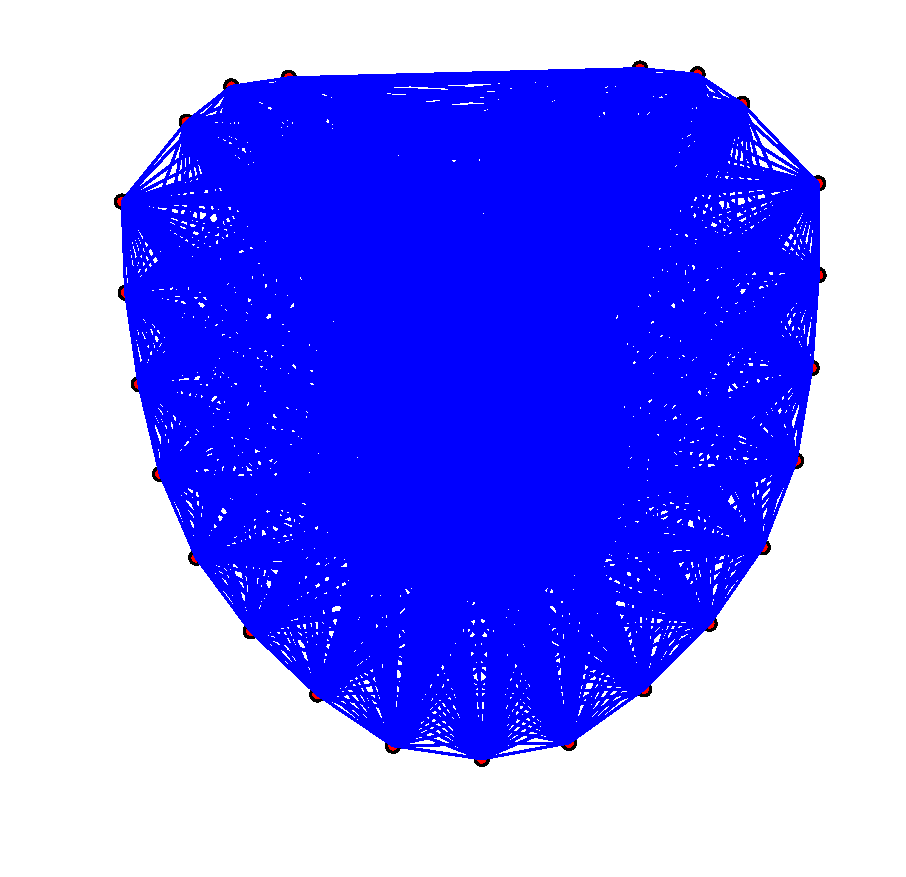
\includegraphics[width=0.3\linewidth]{figures/aps/graphs/full.eps}\label{fig:graph_a}}
  \subfloat[Chain per area]{\includegraphics[width=0.3\linewidth]{figures/aps/graphs/chain_per_area.eps}\label{fig:graph_b}}
  \subfloat[Chain and complete per area]{\includegraphics[width=0.3\linewidth]{figures/aps/graphs/complete_and_chain.eps}\label{fig:graph_c}}\\
  \subfloat[Chain and complete per area with connections between them]{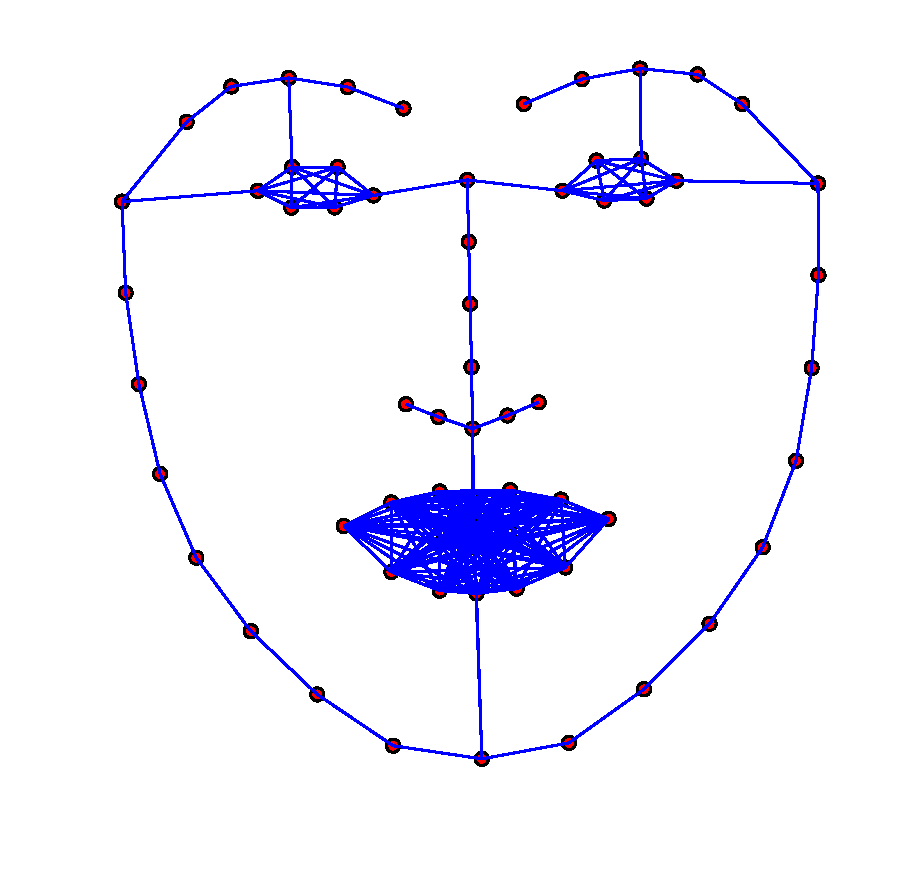
\includegraphics[width=0.3\linewidth]{figures/aps/graphs/joan.eps}\label{fig:graph_d}}
  \subfloat[Minimum spanning tree]{\includegraphics[width=0.3\linewidth]{figures/aps/graphs/mst.eps}\label{fig:graph_e}}
  \subfloat[Empty graph]{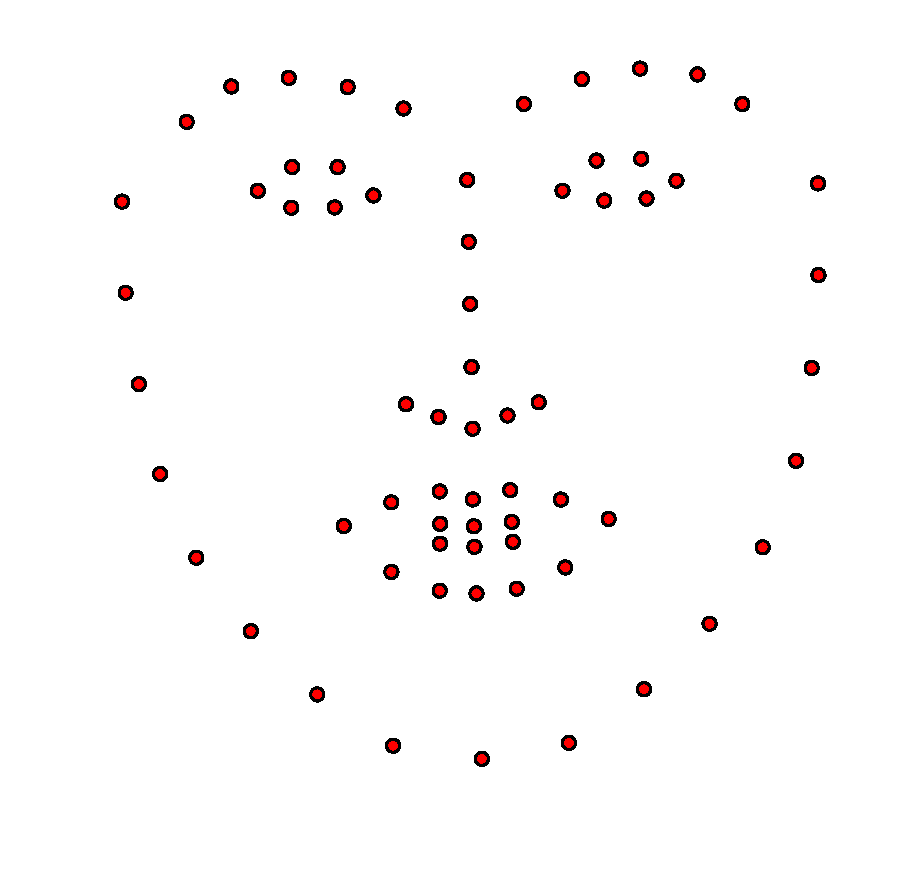
\includegraphics[width=0.3\linewidth]{figures/aps/graphs/diagonal.eps}\label{fig:graph_f}}
  \caption{Employed GMRF graph structures.}
  \label{fig:graphs}
\end{figure}
%
\section{Experimental Results}
\label{sec:aps:exp}
In this section we present a comprehensive evaluation of the different ways in
which APS can be used to model the shape and appearance of an object and
compare their performance against state-of-the-art Deformable Models. In all
presented cases, the proposed APS are built using a two-level pyramid. We keep
about $92\%$ of the shape variance and set $n_a=150$ for both levels that
corresponds to about $80\%$ of the appearance variance. The appearance is
represented either by pixel intensities or dense SIFT~\cite{lowe1999object}
with $8$ channels and the extracted patch size is $17\times17$. The accuracy of
the fitting results is measured by the point-to-point RMS error between the
fitted shape and the ground truth annotations, normalized by the face size, as
proposed in~\cite{zhu2012face}. Note that our Python implementation of
APS runs at $50ms$ per frame, which is very close to real-time. We believe that
with further code optimization, APS are likely to be capable of running in
real-time on high end desktop/laptop machine. Their time complexity is
independent of the graph structure that is employed.

\subsection{Internal Experimental Analysis}\label{sec:aps:internal_results}
Herein, we present three experiments as a proof of concept regarding the
formulation of APS. Specifically, we aim to examine the contribution of each
one of the shape, appearance and deformation models and
\textcolor{red}{\st{find an optimal graph structure} evaluate various graph structures}. 
The model is trained using the 811 images of
LFPW~\cite{belhumeur2011localizing} train set and tested on the corresponding
test set. We use the annotations provided by the 300W
competition~\cite{sagonas2013300,sagonas2013semi,sagonas2016faces} and evaluate
using 66 landmark points which are derived by removing landmarks 61 and 65 from
the 68-points mark-up. In this set of experiments, we don't extract any
appearance features and only use pixel intensities. Figure~\ref{fig:graphs}
shows the graph structures that we employ for the purpose of these experiments.
Note that the minimum spanning tree (MST) is computed as shown
in~\cite{felzenszwalb2005pictorial}. The fitting process of the presented
experiments is initialized by adding Gaussian noise to the global similarity
transform retrieved from the ground truth annotations (without in-plane
rotation) and applying it to the mean shape $\bar{\mathbf{s}}$. We set the
standard deviation of the random noise to 0.04, which generates very
challenging initializations.

%
\begin{table}[!h]
\renewcommand{\arraystretch}{1.3}
\centering
\begin{tabular}{|l|c|c|c|}
\hline
\emph{Graph type $G^a$} & \emph{mean $\pm$ std} & \emph{median} & $\leq 0.04$\\
\hline\hline
Fig.~\ref{fig:graph_a} & 0.0399 $\pm$ 0.0227 & 0.0324 & 68.3\%\\
\textbf{Fig.~\ref{fig:graph_b}} & \textbf{0.0391} $\mathbf{\pm}$ \textbf{0.0243} & \textbf{0.0298} & \textbf{69.6\%}\\
Fig.~\ref{fig:graph_c} & 0.0506 $\pm$ 0.0371 & 0.0370 & 58.9\%\\
Fig.~\ref{fig:graph_d} & 0.0492 $\pm$ 0.0373 & 0.0354 & 58.9\%\\
Fig.~\ref{fig:graph_e} & 0.0413 $\pm$ 0.0257 & 0.0316 & 65.2\%\\
Fig.~\ref{fig:graph_f} & 0.0398 $\pm$ 0.0246 & 0.0319 & 66.5\%\\
\hline\hline
PCA & 0.0716 $\pm$ 0.0454 & 0.0595 & 25.5\%\\
\hline\hline
Initialization & 0.0800 $\pm$ 0.0280 & 0.0768 & 4.0\%\\
\hline
\end{tabular}
\caption{Comparison of the GMRF-based and the PCA-based appearance model of APS.}
\label{tab:appearance_experiment}
\end{table}
%
Beginning with the appearance model, Tab.~\ref{tab:appearance_experiment}
reports the performance when using a GMRF with the graph structures of
Fig.~\ref{fig:graphs} and when using a single multivariate normal distribution
through PCA. The performance is reported in the form of statistical measures
(mean, median and standard deviation) and as the percentage of the testing
images that achieved a final error $\leq0.04$ (value at which the result is
considered adequately good by visual inspection). For this experiment, we use a
PCA shape model and a deformation prior with the MST. The improvement is
significantly high. Even the empty graph, which generates a block diagonal
precision matrix $\mathbf{Q}^a$, thus it assumes independence between all
parts, greatly outperforms the PCA case. The most appropriate graph structure
is the one of Fig.~\ref{fig:graph_b}, which suggests that, for the case of
faces, it is better to connect the landmarks of each facial area (eyes, mouth,
nose etc.) between them and avoid relating the areas between each other.

%
\begin{table}[!h]
\renewcommand{\arraystretch}{1.3}
\centering
\begin{tabular}{|l|c|c|c|}
\hline
\emph{Graph type $G^s$} & \emph{mean $\pm$ std} & \emph{median} & $\leq 0.04$\\
\hline\hline
Fig.~\ref{fig:graph_a} & 0.0495 $\pm$ 0.0273 & 0.0420 & 45.5\%\\
Fig.~\ref{fig:graph_b} & 0.0496 $\pm$ 0.0276 & 0.0438 & 45.5\%\\
Fig.~\ref{fig:graph_c} & 0.0503 $\pm$ 0.0262 & 0.0433 & 44.2\%\\
Fig.~\ref{fig:graph_d} & 0.0495 $\pm$ 0.0257 & 0.0434 & 44.6\%\\
Fig.~\ref{fig:graph_e} & 0.0519 $\pm$ 0.0306 & 0.0437 & 43.8\%\\
Fig.~\ref{fig:graph_f} & 0.0492 $\pm$ 0.0249 & 0.0437 & 42.9\%\\
\hline\hline
\textbf{PCA} & \textbf{0.0412} $\mathbf{\pm}$ \textbf{0.0295} & \textbf{0.0301} & \textbf{65.6\%}\\
\hline\hline
Initialization & 0.0800 $\pm$ 0.0280 & 0.0768 & 4.0\%\\
\hline
\end{tabular}
\caption{Comparison of the GMRF-based and the PCA-based shape model of APS.}
\label{tab:shape_experiment}
\end{table}
%
Table~\ref{tab:shape_experiment} presents the same experiment for the shape
model and the results are opposite to those of the appearance model. However,
this is a well expected result. As mentioned in Sec.~\ref{subsec:aps:training},
the appearance model utilizes directly the constructed block sparse precision
matrix. On the contrary, we need to decompose the covariance matrix
($\boldsymbol{\Sigma}^s=(\mathbf{Q}^s)^{-1}$) of the shape model in order to
learn a parametric subspace that will be used during optimization. However, due
to the block sparse formulation, the resulting covariance matrix has high (in
some cases full) rank. Most eigenvalues are non-zero and they represent a small
percentage of the data variance.
%Figure~\ref{fig:spectrums} shows the spectrum of the covariance matrices of Tab.~\ref{tab:shape_experiment}.
Thus by keeping more than $90\%$ of the total variance, the model ends up with
too many modes of variation (about 100 in the case of 68 vertexes and depending
on the graph structure). Consequently, it is very hard to apply a robust
optimization in such a parametric space, as the search space is too large.

%
\begin{table}[!h]
\renewcommand{\arraystretch}{1.3}
\centering
\begin{tabular}{|l||c|c|}
\hline
\emph{Deformation} & \multicolumn{2}{c|}{Shape model $G^s$}\\
\cline{2-3}
\emph{prior $G^d$} & \emph{Fig.~\ref{fig:graph_a}}  & \emph{PCA}\\
\hline\hline
No prior & 0.1327 $\pm$ 0.0857 & 0.0429 $\pm$ 0.0267\\
Fig.~\ref{fig:graph_b} & 0.0524 $\pm$ 0.0256 & 0.0430 $\pm$ 0.0240\\
\textbf{Fig.~\ref{fig:graph_e}} & \textbf{0.0495} $\mathbf{\pm}$ \textbf{0.0273} & \textbf{0.0391} $\mathbf{\pm}$ \textbf{0.0243}\\
\hline
\end{tabular}
\caption{Comparison of the GMRF-based and the PCA-based deformation prior of APS in combination with the GMRF-based and the PCA-based shape model.}
\label{tab:deformation_experiment}
\end{table}
%
Finally, Tab.~\ref{tab:deformation_experiment} examines the contribution of the deformation prior of Eq.~\ref{equ:cost_function}. We use the graph of Fig.~\ref{fig:graph_b} for the appearance model and we test for two cases of the shape model: PCA and GMRF with a complete graph (Fig.~\ref{fig:graph_a}). The results prove that the prior plays an important role in both cases, as it improves the result. Especially in the case of the GMRF, the improvement is significant. Given the previous analysis about the non robust behavior of a GMRF shape model, this result is expected because the prior term will prevent the shape model from generating non-realistic instances of the face.

%
\begin{figure}[!t]
  \centering
  \hspace{0.5cm}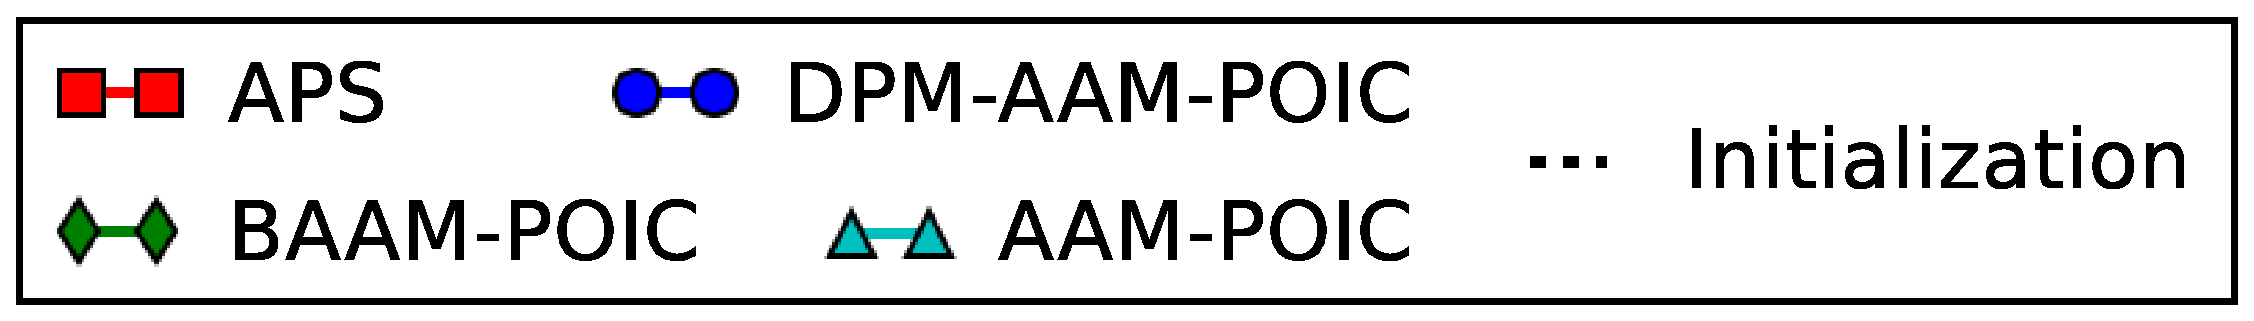
\includegraphics[height=0.95cm]{figures/aps/legend1/legend.eps}
  \subfloat[Accuracy]{\includegraphics[width=0.58\linewidth]{figures/aps/inverse_comparison/inverse_comparison.eps}\label{fig:inverse_comparison}}\\
  \subfloat[Convergence]{\includegraphics[width=0.58\linewidth]{figures/aps/inverse_comparison/convergence.eps}\label{fig:convergence}}
  \caption{Comparison of APS accuracy and convergence with other inverse compositional methods with fixed Jacobian and Hessian on AFW database. The dashed vertical black line in \emph{(b)} denotes the transition from lower to higher pyramidal level.}
\end{figure}
%
\subsection{Comparison with State-of-the-Art Methods}\label{sec:aps:comparison}
Figures~\ref{fig:inverse_comparison} and~\ref{fig:convergence} aim to compare
the accuracy and convergence speed of APS against the other existing inverse
compositional techniques with fixed Jacobian and Hessian (POIC) mentioned
in~\ref{sec:derivation}. AAM-POIC~\cite{matthews2004active} and
BAAM-POIC~\cite{alabort2014bayesian} denote the POIC optimization of an AAM and
a Bayesian AAM. AAM-DPM-POIC refers to the inverse algorithm that can be
combined with the AAM part-based model of~\cite{tzimiropoulos2014gauss}. All
methods are trained on LFPW database in the same manner, using the same pyramid
and extracting dense SIFT features with 8 channels. For all of them we keep
$n_s=5$ and $n_s=15$ shape components for the low and high levels respectively,
that correspond to about $92\%$ of the total shape variance, and $n_a=150$
appearance components for both levels. The results, which are computed using 66
landmark points, are reported on the challenging AFW~\cite{zhu2012face}
database and indicate that the proposed method outperforms all existing
inverse-compositional techniques by a significant margin. Most importantly, APS
need very few number of iterations in order to converge (less than 10 at the
first pyramidal level and no more than 4 at the second), which highlights their
close to real-time computational complexity.

%
\begin{figure}[!t]
  \centering
  \hspace{0.5cm}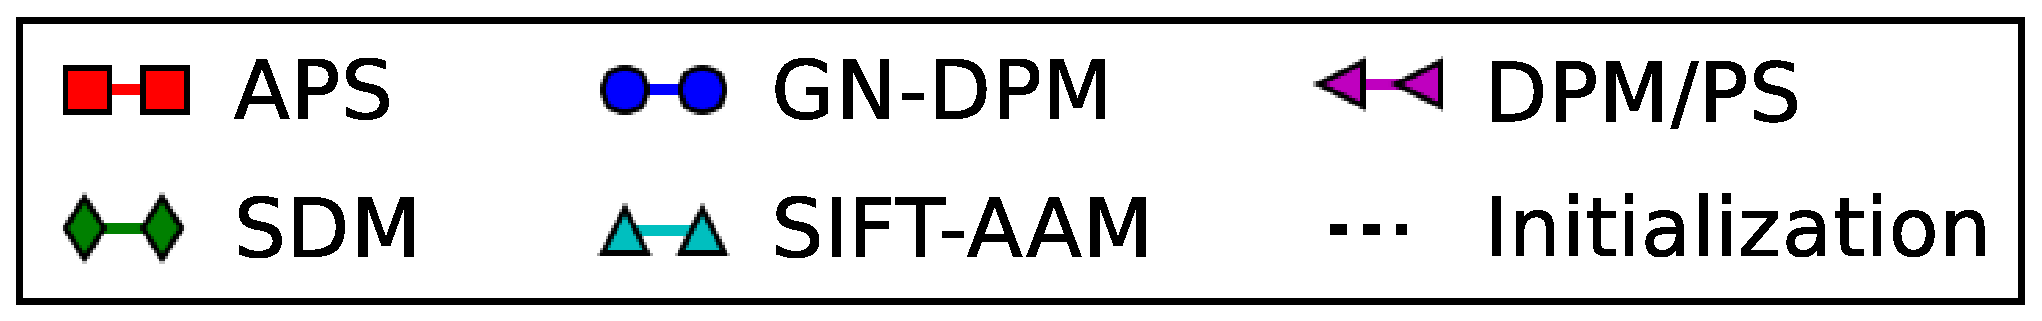
\includegraphics[height=0.95cm]{figures/aps/legend2/legend.eps}\vspace{0.3cm}\\
  \includegraphics[width=0.58\linewidth]{figures/aps/state-of-the-art.eps}
  \caption{Comparison of APS with current state-of-the-art methods on AFW database.}
  \label{fig:aps:state_of_the_art}
\end{figure}
%
%
\begin{table}[!t]
\renewcommand{\arraystretch}{1.3}
\centering
\begin{tabular}{|c|c|c|c|c|}
\hline
\emph{APS} & \emph{SDM} & \emph{SIFT-AAM} & \emph{GN-DPM} & \emph{DPM/PS}\\
\hline\hline
\textbf{0.0415} & 0.0453 & 0.0423 & 0.0686 & 0.0585\\
\hline
\end{tabular}
\caption{Mean values of the cumulative error curves reported in Fig.~\ref{fig:aps:state_of_the_art}.}
\label{tab:aps:state_mean}
\end{table}
%
Figure~\ref{fig:aps:state_of_the_art} compares APS against the current
state-of-the-art techniques: SDM~\cite{xiong2013supervised}, the recently
proposed GN-DPM~\cite{tzimiropoulos2014gauss} and
SIFT-AAM~\cite{antonakos2014hog,antonakos2015feature}. The initialization for
all methods is done using the bounding box of the landmark points returned by
DPM~\cite{zhu2012face} (the black dashed line). For all the methods we used the
pre-trained implementations provided by their authors, except SIFT-AAM which we
trained using the Menpo Project~\cite{menpo2014}. Note that all competing
methods are trained on much more data than the 811 LFPW images that we use. The
result is reported on the AFW database and computed based on 49 points, which
is the mark-up that both SDM and GN-DPM return. Table~\ref{tab:aps:state_mean}
reports the mean values of the cumulative error curves of
Fig.~\ref{fig:aps:state_of_the_art}. These results show that APS outperform all
methods and are more robust. Note that GN-DPM is very accurate when the
initialization is close to the ground-truth but is not robust against bad
initializations, as indicated by its large mean error value. Finally,
Fig.~\ref{fig:aps:faces_examples} shows some indicative fitting examples.



%
\begin{figure}[!h]
  \centering
  \subfloat[Initialization]{
  \includegraphics[width=0.19\linewidth]{figures/aps/faces/face1_1.eps}
  \includegraphics[width=0.19\linewidth]{figures/aps/faces/face2_1.eps}
  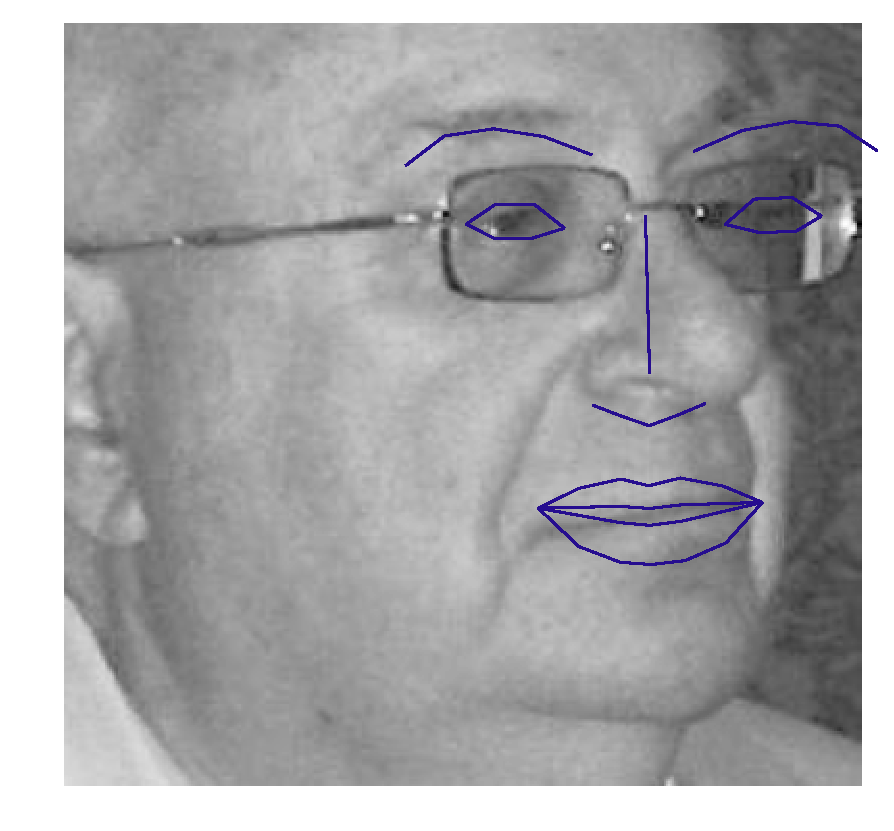
\includegraphics[width=0.19\linewidth]{figures/aps/faces/face3_1.eps}
  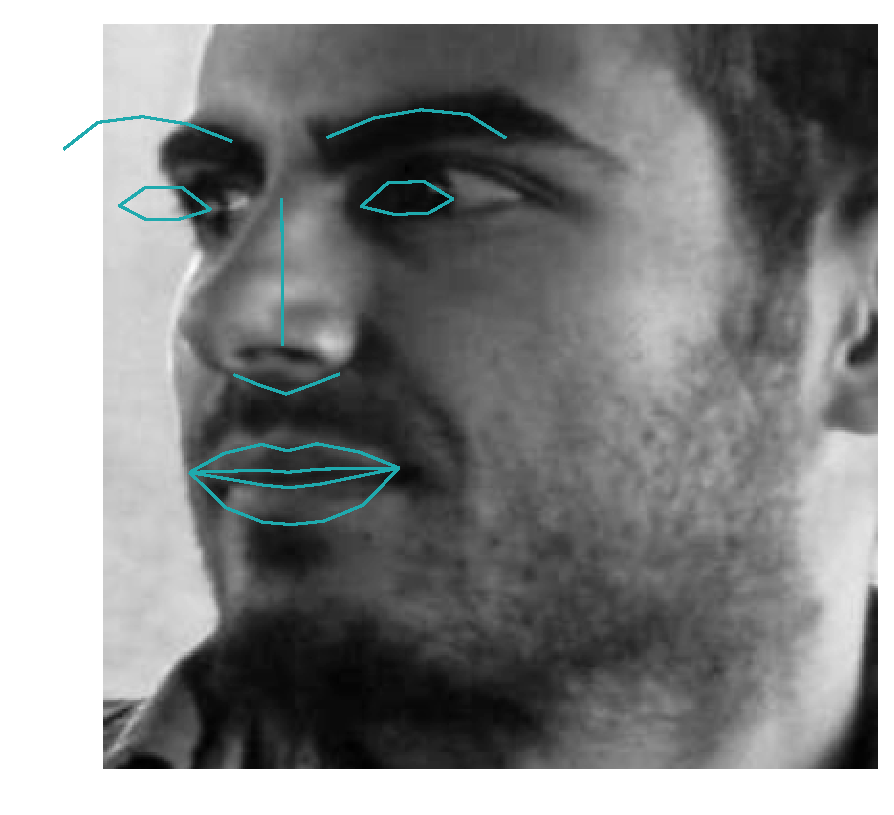
\includegraphics[width=0.19\linewidth]{figures/aps/faces/face4_1.eps}
  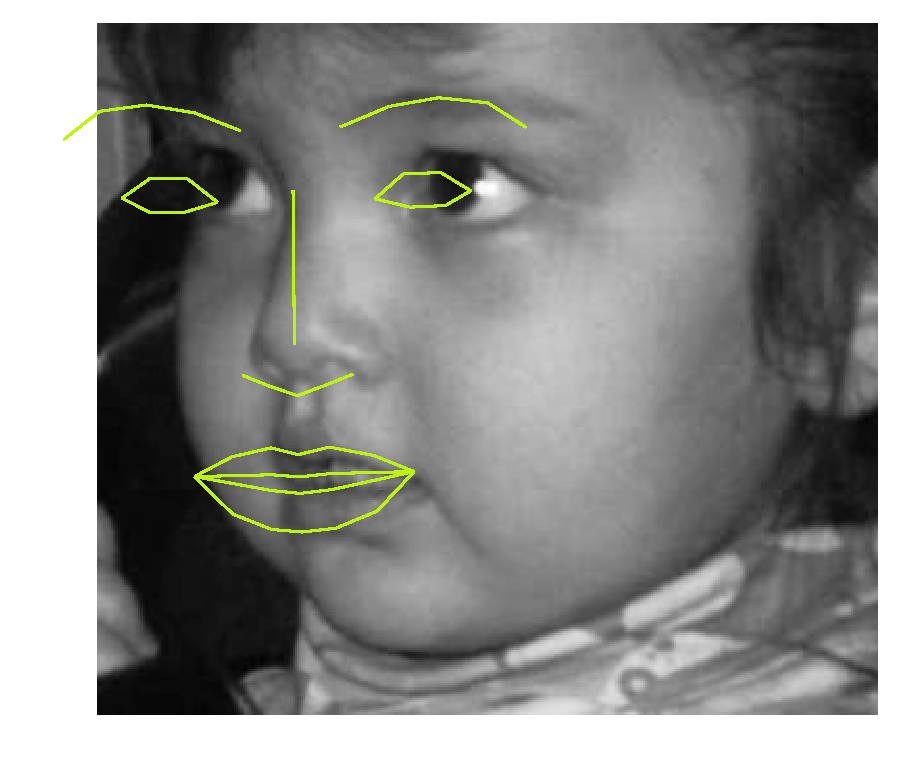
\includegraphics[width=0.19\linewidth]{figures/aps/faces/face5_1.eps}}\\
  \subfloat[Final fitting]{
  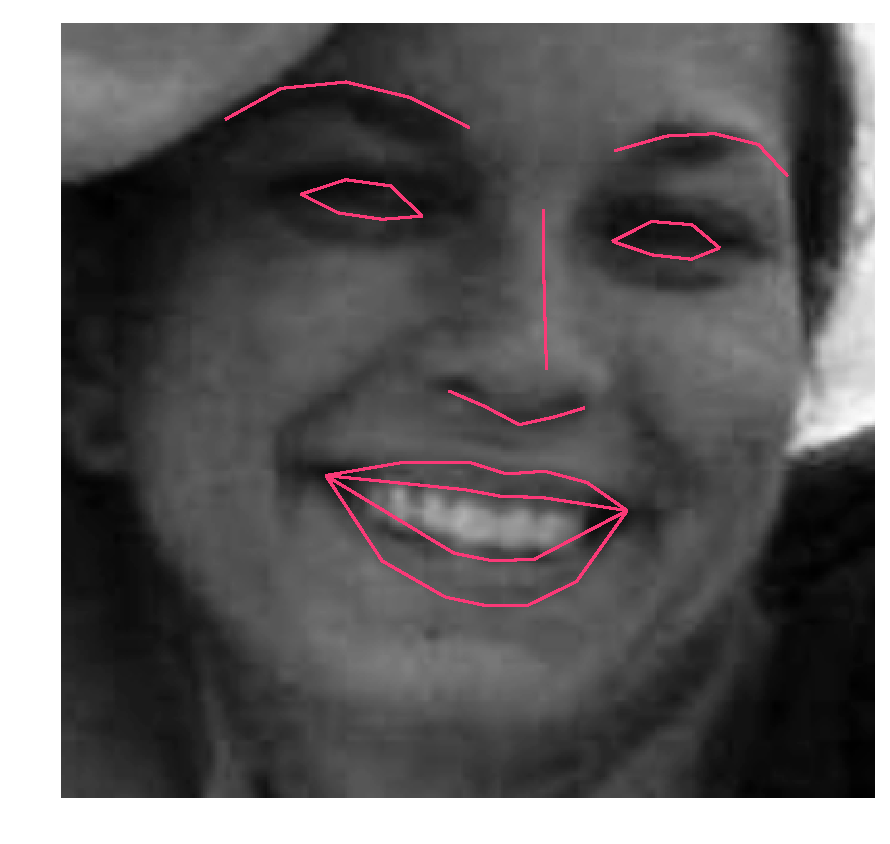
\includegraphics[width=0.19\linewidth]{figures/aps/faces/face1_2.eps}
  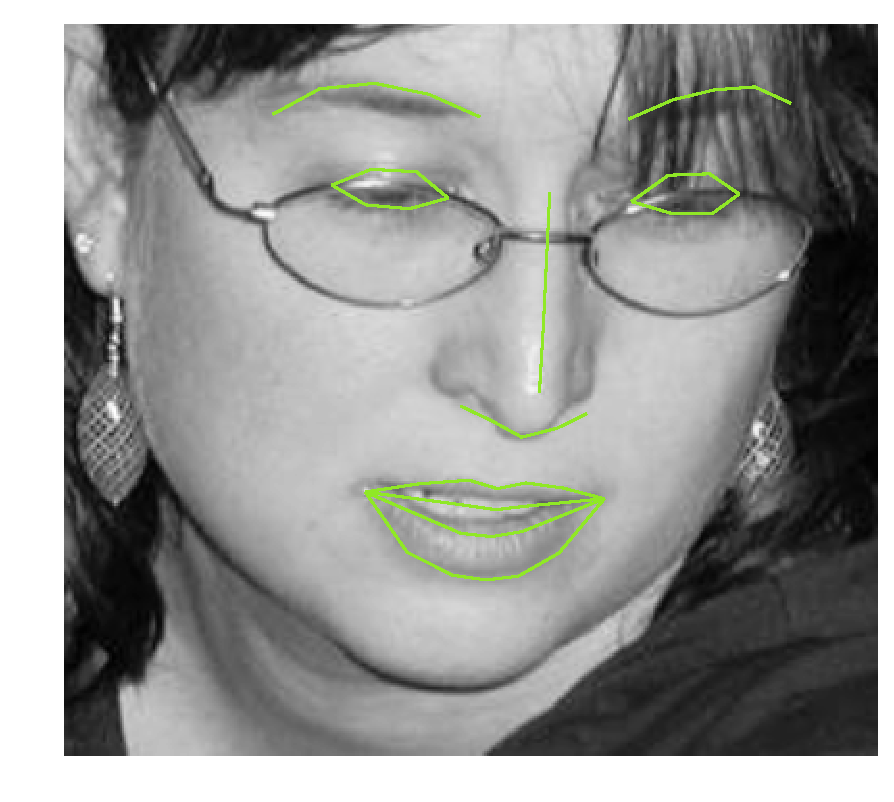
\includegraphics[width=0.19\linewidth]{figures/aps/faces/face2_2.eps}
  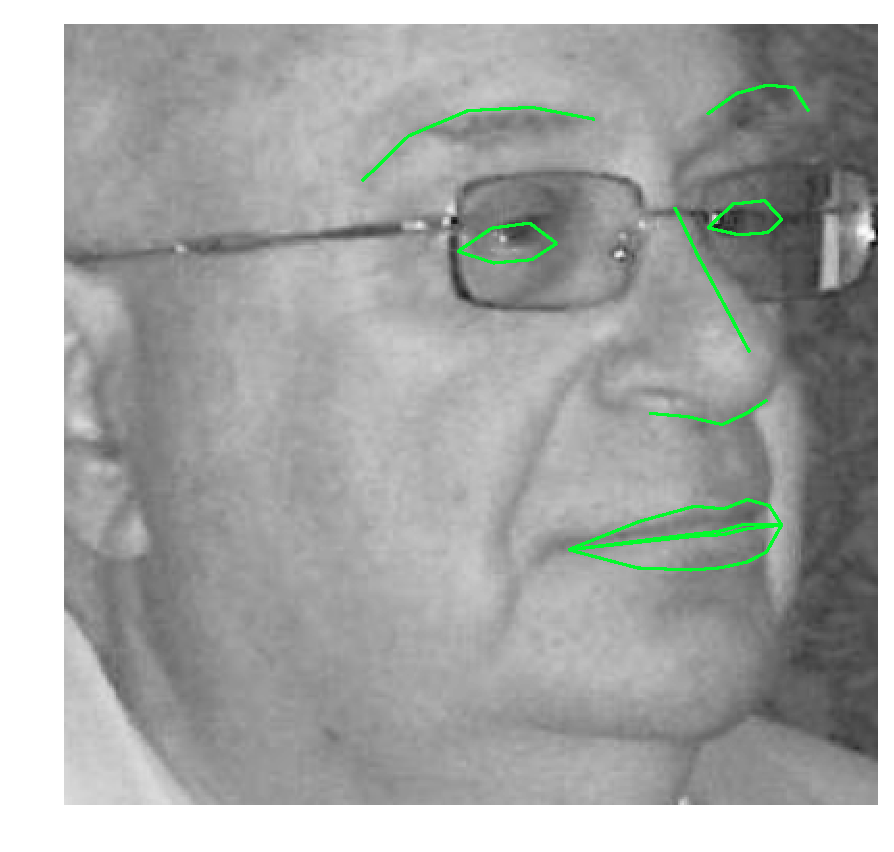
\includegraphics[width=0.19\linewidth]{figures/aps/faces/face3_2.eps}
  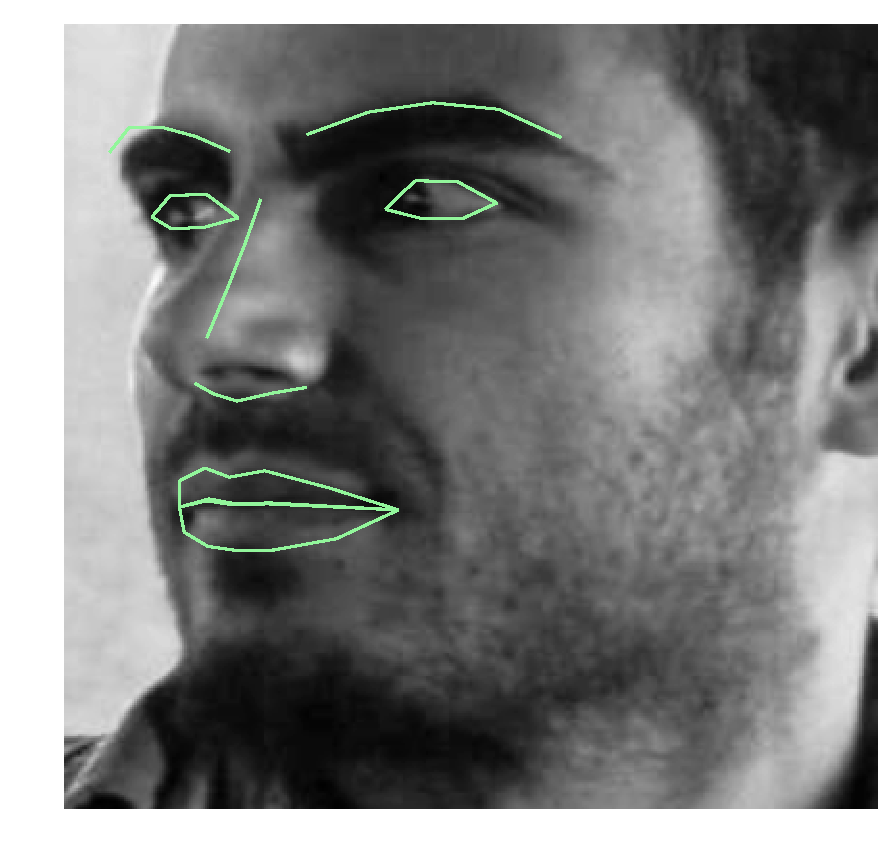
\includegraphics[width=0.19\linewidth]{figures/aps/faces/face4_2.eps}
  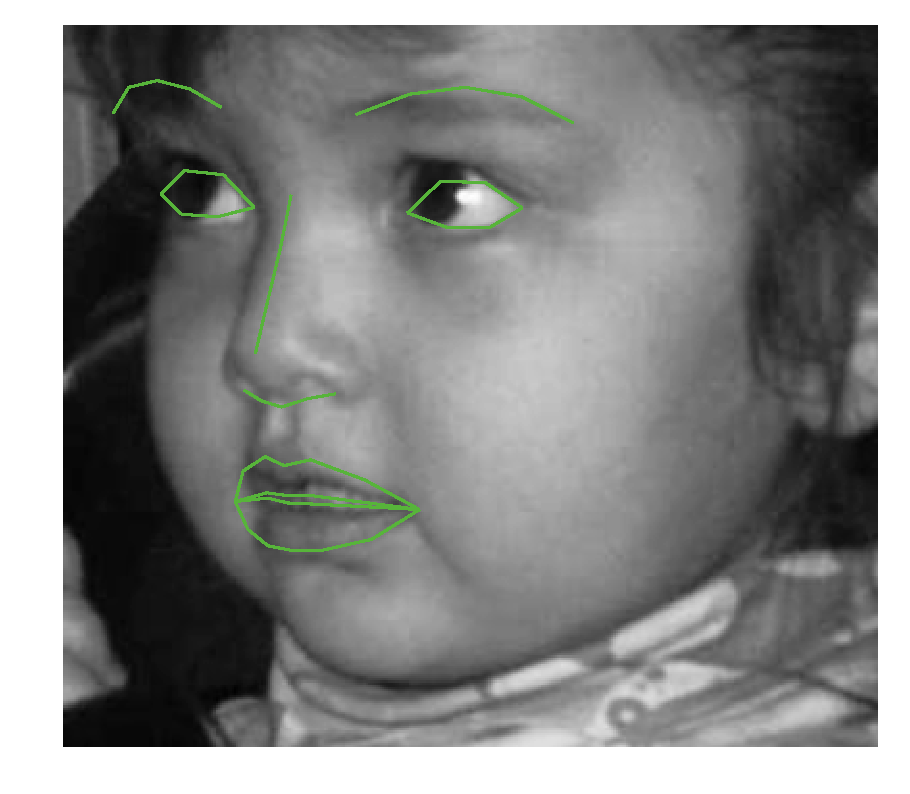
\includegraphics[width=0.19\linewidth]{figures/aps/faces/face5_2.eps}}
  \caption{Fitting results on the AFW facial database. These are indicative results that correspond to the curve of Fig.~\ref{fig:aps:state_of_the_art}.}
  \label{fig:aps:faces_examples}
\end{figure}
%

\subsection{Results on Other Deformable Objects}
Note that APS is a flexible patch-based Deformable Model that can also be
applied to the landmark localization of other objects. Herein, we show
indicative results for the case of eyes and cars. In the case of cars, we
employ the sideview (view 2) images from CMU
database~\cite{boddeti2013correlation,li2011robustly}, which we split in 450
and 151 training and testing images, respectively. For eyes, we use our
in-house annotated database that consists of 38 manually annotated landmarks
and it has 600 and 400 training and testing images respectively. Figure~\ref{fig:curves} shows the cumulative fitting error curves for both
objects. For the initialization, we add Gaussian noise to the global similarity
transform retrieved from the ground-truth annotations (without in-plane
rotation) and apply it to the mean shape of the object. The standard deviation
of the noise is set to 0.06.
%
\begin{figure}[!h]
  \centering
  \subfloat[Eyes]{\includegraphics[width=0.49\linewidth]{figures/aps/eyes/eye.eps}\label{fig:eyes}}
  \subfloat[Cars]{\includegraphics[width=0.49\linewidth]{figures/aps/cars/car.eps}\label{fig:cars}}
  \caption{Fitting results of APS for human eyes and cars.}
  \label{fig:curves}
\end{figure}
%

Finally, Figs.~\ref{fig:eyes_examples} and~\ref{fig:cars_examples} show some
indicative fitting examples for both objects. Note that in the case of human
eyes, most of the error is accumulated by the should be the upper and lower
sclera, because it is a region without any distinctive features.

%
\begin{figure}[!h]
  \centering
  \subfloat[Initialization]{
  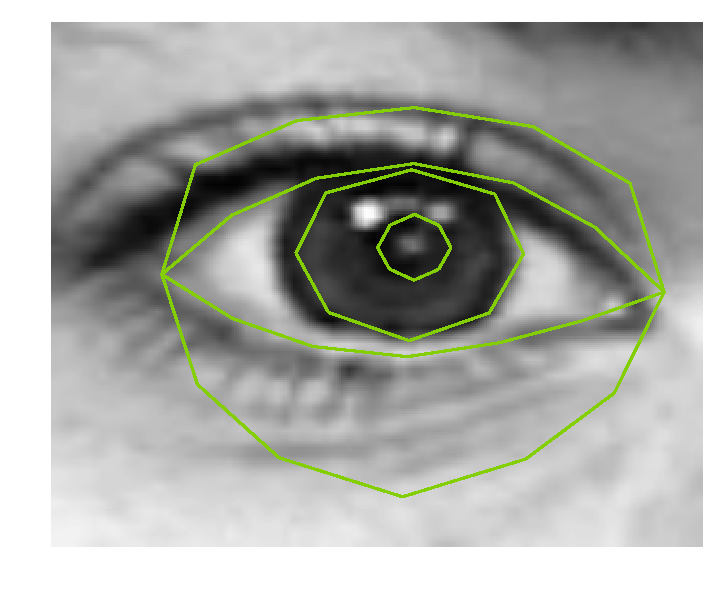
\includegraphics[width=0.19\linewidth]{figures/aps/eyes/eye1_1.eps}
  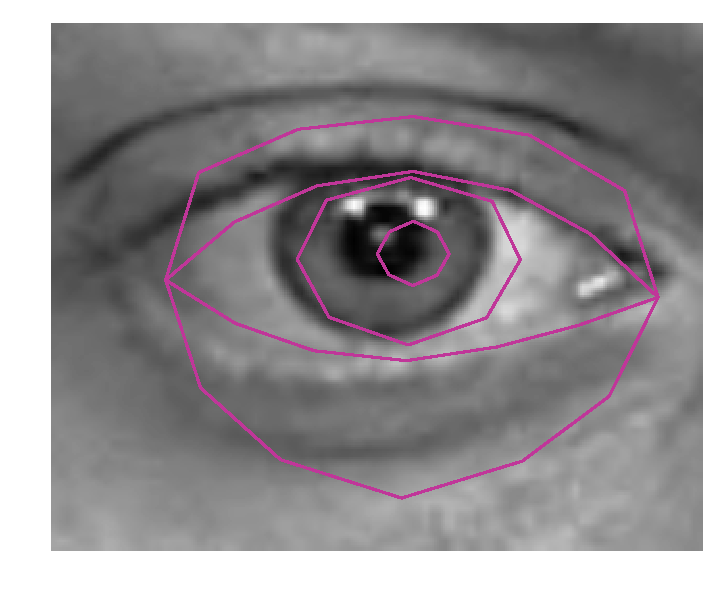
\includegraphics[width=0.19\linewidth]{figures/aps/eyes/eye2_1.eps}
  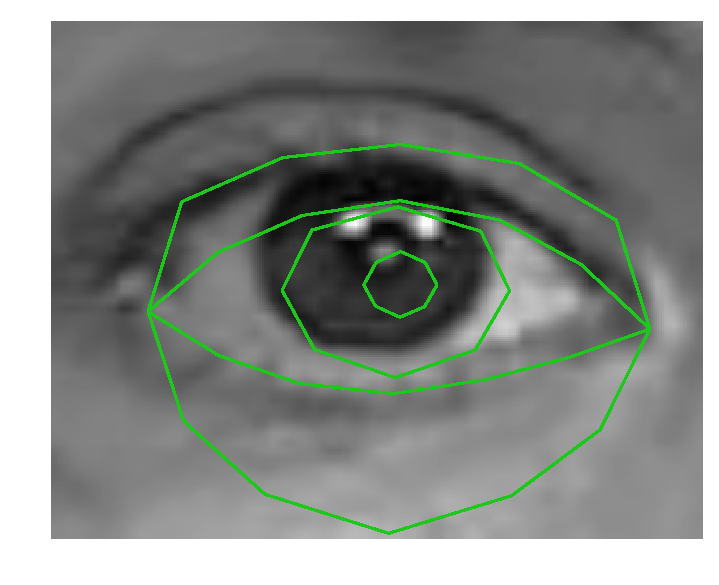
\includegraphics[width=0.19\linewidth]{figures/aps/eyes/eye3_1.eps}
  \includegraphics[width=0.19\linewidth]{figures/aps/eyes/eye4_1.eps}
  \includegraphics[width=0.19\linewidth]{figures/aps/eyes/eye5_1.eps}}\\
  \subfloat[Final fitting]{
  \includegraphics[width=0.19\linewidth]{figures/aps/eyes/eye1_2.eps}
  \includegraphics[width=0.19\linewidth]{figures/aps/eyes/eye2_2.eps}
  \includegraphics[width=0.19\linewidth]{figures/aps/eyes/eye3_2.eps}
  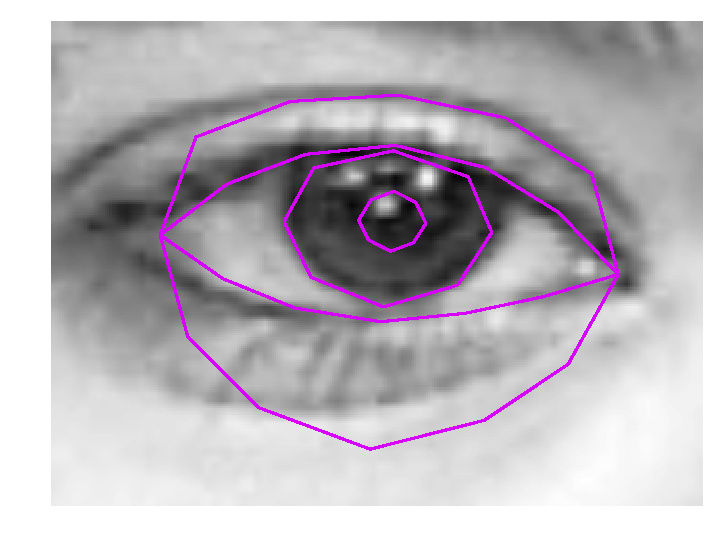
\includegraphics[width=0.19\linewidth]{figures/aps/eyes/eye4_2.eps}
  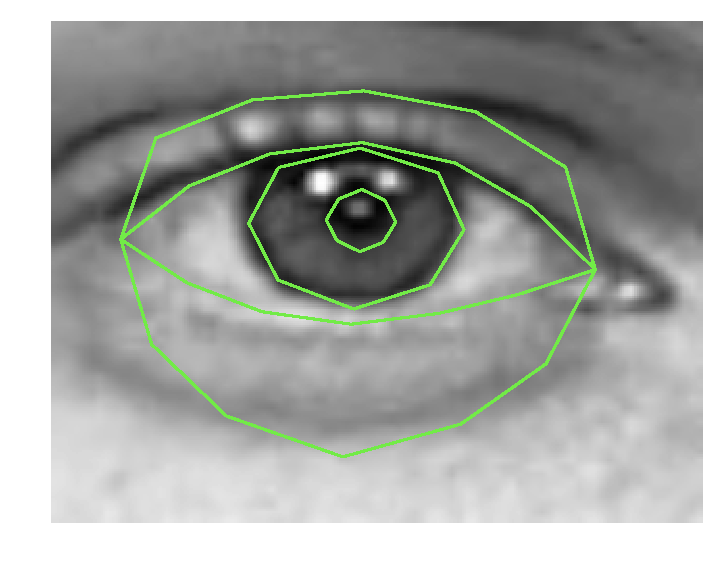
\includegraphics[width=0.19\linewidth]{figures/aps/eyes/eye5_2.eps}}
  \caption{Fitting results on open eyes. These are indicative results that correspond to the curve of Fig.~\ref{fig:eyes}.}
  \label{fig:eyes_examples}
\end{figure}
%

%
\begin{figure}[!h]
  \centering
  \subfloat[Initialization]{
  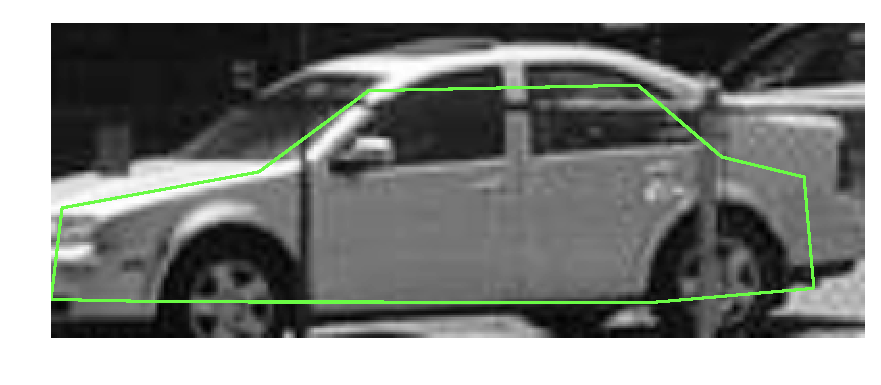
\includegraphics[width=0.19\linewidth]{figures/aps/cars/car1_1.eps}
  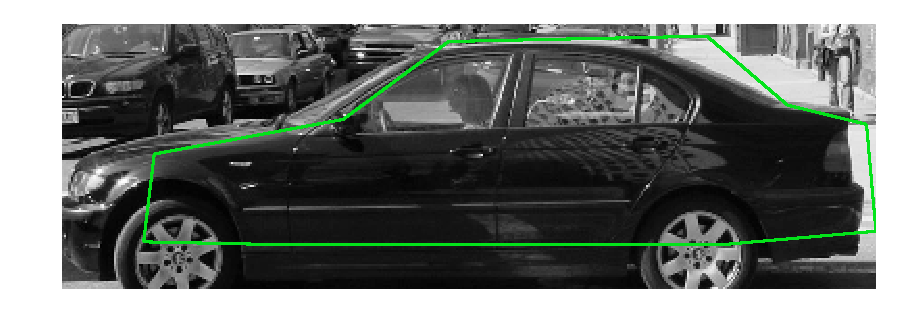
\includegraphics[width=0.19\linewidth]{figures/aps/cars/car2_1.eps}
  \includegraphics[width=0.19\linewidth]{figures/aps/cars/car3_1.eps}
  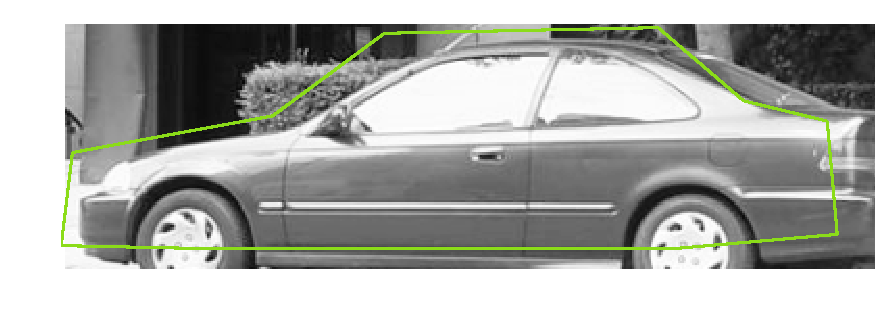
\includegraphics[width=0.19\linewidth]{figures/aps/cars/car4_1.eps}
  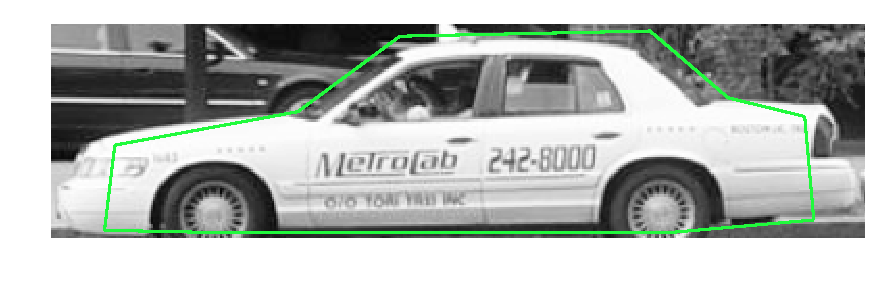
\includegraphics[width=0.19\linewidth]{figures/aps/cars/car5_1.eps}}\\
  \subfloat[Final fitting]{
  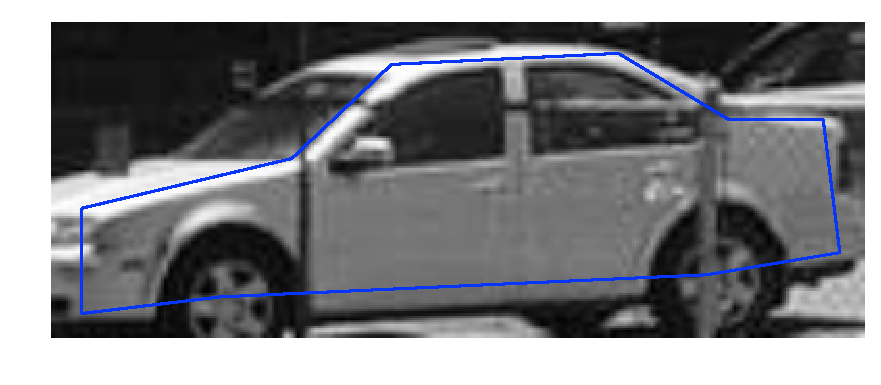
\includegraphics[width=0.19\linewidth]{figures/aps/cars/car1_2.eps}
  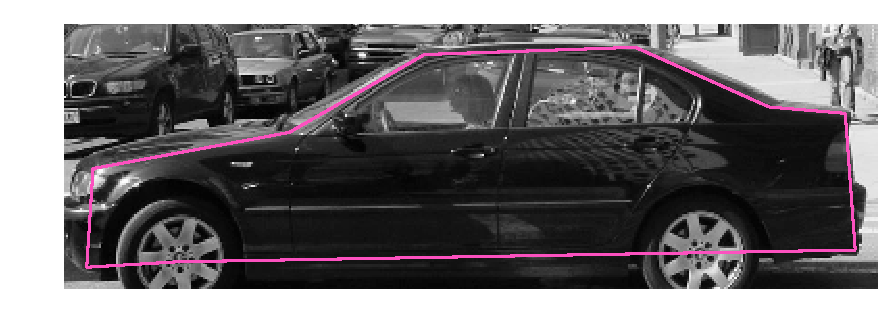
\includegraphics[width=0.19\linewidth]{figures/aps/cars/car2_2.eps}
  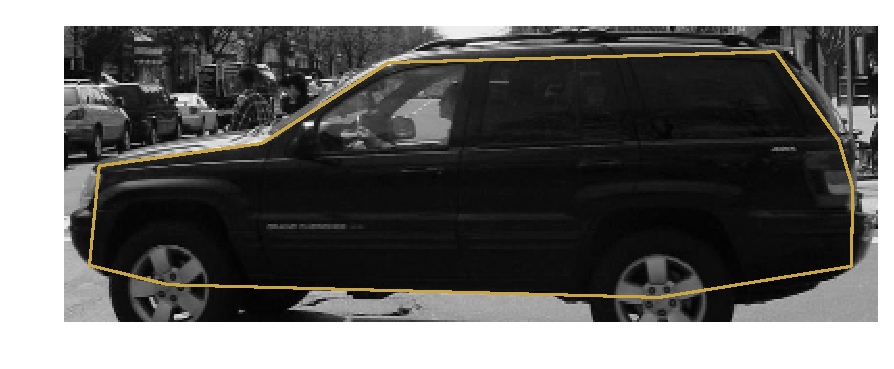
\includegraphics[width=0.19\linewidth]{figures/aps/cars/car3_2.eps}
  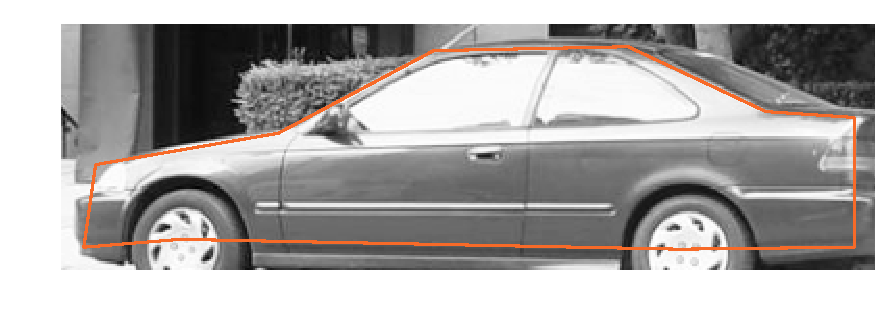
\includegraphics[width=0.19\linewidth]{figures/aps/cars/car4_2.eps}
  \includegraphics[width=0.19\linewidth]{figures/aps/cars/car5_2.eps}}
  \caption{Fitting results on cars sideview. These are indicative results that correspond to the curve of Fig.~\ref{fig:cars}.}
  \label{fig:cars_examples}
\end{figure}
%
